\section{Implementatie}
In \cref{sec:ontwerp} is voor elk onderdeel van het systeem besproken wat de eisen zijn van dat onderdeel. Dit hoofdstuk gaat in op de implementatie van elk van deze systeemonderdelen.

\subsection{Spanningsreferentie}
Zoals besproken in \cref{sec:referenceVoltage} kunnen de weerstandswaardes van de spanningsreferentie erg hoog gekozen worden. Met een $R_1$ van \qty{5.6}{\mega\ohm} gebruikt de spanningsdeler \qty{1.65}{\micro\watt}.

Volgens \cref{eq:dividerNoise} heeft de condensatorwaarde wel effect op de ruis. Met een condensator van \qty{1}{\micro\farad} produceert de spanningsreferentie \qty{64.4}{\nano\volt} aan ruis. Dit zorgt voor een signaal-ruis verhouding van \qty{138}{\decibel}, wat meer dan genoeg is.

Deze gekozen waardes en de resulterende eigenschappen zijn te vinden in \cref{tab:divider}.

\begin{table}[!htbp]
    \centering
    \begin{tabular}{l|l|l}
        Symbool & Waarde & Eenheid \\
        \hline
        $R_1$       & 5.6  & $\si{\mega\ohm}$   \\
        $R_2$       & 1.0  & $\si{\mega\ohm}$   \\
        $C$         & 1.0  & $\si{\micro\farad}$\\
        $P$         & 1.65 & $\si{\micro\watt}$ \\
        $u_{n,out}$ & 64.4 & $\si{\nano\volt}$  \\
        SNR         & 138  & $\si{\decibel}$
    \end{tabular}
    \caption{De gekozen waardes van de spanningsdeler, met het resulterende vermogensverbruik en de ruiseigenschappen.}
    \label{tab:divider}
\end{table}

\begin{figure}[!htbp]
    \centering
    \def\svgwidth{7cm}
    \subsection{Spanningsreferentie}\label{sec:referenceVoltage}

De ISFET uitleesschakeling heeft een spanningsreferentie nodig om te werken.
% TODO: Vertel misschien over andere methoden.
Hiervoor is als implementatie een spanningsdeler gekozen. De schakeling van deze spanningsdeler is te zien in \cref{fig:divider}.
De condensator wordt gebruikt om ruis te verminderen op hogere frequenties, en dient ook als filter voor hoogfrequente storing in de voedingsspanning.

\begin{figure}[!htbp]
    \centering
    \def\svgwidth{0.5\textwidth}
    \subsection{Spanningsreferentie}\label{sec:referenceVoltage}

De ISFET uitleesschakeling heeft een spanningsreferentie nodig om te werken.
% TODO: Vertel misschien over andere methoden.
Hiervoor is als implementatie een spanningsdeler gekozen. De schakeling van deze spanningsdeler is te zien in \cref{fig:divider}.
De condensator wordt gebruikt om ruis te verminderen op hogere frequenties, en dient ook als filter voor hoogfrequente storing in de voedingsspanning.

\begin{figure}[!htbp]
    \centering
    \def\svgwidth{0.5\textwidth}
    \subsection{Spanningsreferentie}\label{sec:referenceVoltage}

De ISFET uitleesschakeling heeft een spanningsreferentie nodig om te werken.
% TODO: Vertel misschien over andere methoden.
Hiervoor is als implementatie een spanningsdeler gekozen. De schakeling van deze spanningsdeler is te zien in \cref{fig:divider}.
De condensator wordt gebruikt om ruis te verminderen op hogere frequenties, en dient ook als filter voor hoogfrequente storing in de voedingsspanning.

\begin{figure}[!htbp]
    \centering
    \def\svgwidth{0.5\textwidth}
    \input{img/divider.pdf_tex}
    \caption{De schakeling van de spanningsdeler die dient als spanningsreferentie.}
    \label{fig:divider}
\end{figure}

De overdracht van deze spanningsdeler is te vinden in \cref{eq:dividerTransfer}.
\begin{equation}\label{eq:dividerTransfer}
    H(s) = \frac{U_{ref}(s)}{U_{dd}(s)} = \frac{R_2}{R_1 + R_2 + R_2Cs}
\end{equation}

\subsubsection{Vermogen}
Het vermogen dat de spanningsdeler dissipeert, kan met \cref{eq:dividerPower} berekend worden.
\begin{equation}\label{eq:dividerPower}
    P(s) = U_{dd}^2(s)\frac{1+R_2Cs}{R_1 + R_2 + R_1R_2Cs}
    \tagaddtext{[\si{\watt}]}
\end{equation}
Met een constante DC ingangsspanning kan dit vereenvoudigd worden naar \cref{eq:dividerPowerSimple}.
\begin{equation}\label{eq:dividerPowerSimple}
    P = \frac{U_{dd}^2}{R_1 + R_2}
    \tagaddtext{[\si{\watt}]}
\end{equation}

\subsubsection{Ruis}
Om de ruis van deze schakeling te berekenen moet een aantal stappen genomen worden. Aangezien de ingangsbron $U_{dd}$ een spanningsbron is, kan deze als kortsluiting genomen worden. Op deze manier kunnen de twee weerstanden parallel genomen worden, en verandert de schakeling in een simpel RC filter. In \cref{fig:dividerNoise} is deze omgebouwde schakeling te zien.

\begin{figure}[!htbp]
    \centering
    \def\svgwidth{0.35\textwidth}
    \input{img/dividerNoise.pdf_tex}
    \caption{De omgebouwde schakeling om ruis mee te berekenen.}
    \label{fig:dividerNoise}
\end{figure}

\noindent
Voor de spectrale spanningsruisdichtheid aan de uitgang $U_{ref}$ kan \cref{eq:dividerNoiseLaplace} worden opgesteld.
\begin{equation}\label{eq:dividerNoiseLaplace}
    S_{n,u_{ref}} = 4kTR_e\left(\frac{1}{1 + R_eCs}\right)^2
    \tagaddtext{[\si{\volt\squared\per\hertz}]}
\end{equation}
Wanneer de absolute waarde van de ruis wordt genomen, kan deze over de bandbreedte geïntegreerd worden. Dit resulteert in \cref{eq:dividerNoiseInt}, waar B de bandbreedte is.
\begin{equation}\label{eq:dividerNoiseInt}
    u_{n,ref}^2 = 4kTR_e\int_{B} \frac{1}{1 + (2\pi f R_e C)^2} df
    \tagaddtext{[\si{\volt\squared}]}
\end{equation}
Met een oneindige bandbreedte komt deze integraal uit op \cref{eq:dividerNoiseIntegratedInf}.
\begin{equation}\label{eq:dividerNoiseIntegratedInf}
    u_{n,ref}^2 = \lim_{f\rightarrow\infty}\frac{2kT}{\pi C} \arctan(2\pi f R_eC)
    \tagaddtext{[\si{\volt\squared}]}
\end{equation}
Aangezien de inverse tangens $\frac{\pi}{2}$ nadert, komt dit limiet uit op \cref{eq:dividerNoise}.
\begin{equation}\label{eq:dividerNoise}
    u_{n,ref}^2 = \frac{kT}{C}
    \tagaddtext{[\si{\volt\squared}]}
\end{equation}
Omdat een oneindige bandbreedte gebruikt is om op \cref{eq:dividerNoise} te komen, berekend deze de ruis in het ergste geval. De weerstandswaardes van $R_1$ en $R_2$ zijn hierbij irrelevant. Hierdoor is ruis geen bepalende factor meer tijdens het kiezen van de weerstandswaardes van de spanningsdeler, en kunnen deze volledig gebaseerd worden op vermogensverbruik. Volgens \cref{eq:dividerPowerSimple} is het vermogen omgekeerd evenredig met de som van de weerstandswaardes. Daarbij zit de uitgang van de spanningsdeler direct verbonden met de ingang van een nullor. Er hoeft dus geen rekening gehouden te worden met de uitgangsimpedantie van de spanningsbron. Hierdoor is het voor het vermogensverbruik voordelig om de weerstandswaardes zo hoog mogelijk te kiezen.

\subsubsection{Simulatie}

Om te verifiëren dat de spanningsreferentie goed werkt, is er een aantal simulaties uitgevoerd.

In \cref{fig:referenceSimFreq} is het resultaat van een AC simulatie te zien. Hier is $H(f)$ de overdracht van $U_{dd}$ naar

\begin{figure}[!htbp]
    \centering
    \pgfplotsset{width=0.7\textwidth}
    \input{plots/referenceSimFreq.tex}
    \caption{Het resultaat van een AC simulatie van de spanningsreferentie.}
    \label{fig:referenceSimFreq}
\end{figure}


\begin{figure}[!htbp]
    \centering
    \pgfplotsset{width=0.7\textwidth}
    \input{plots/referenceSimTrans.tex}
    \caption{Het resultaat van een transient simulatie van de spanningsreferentie.}
    \label{fig:referenceSimTrans}
\end{figure}


\begin{figure}[!htbp]
    \centering
    \pgfplotsset{width=0.7\textwidth}
    \input{plots/referenceSimNoise.tex}
    \caption{Het resultaat van een ruissimulatie van de spanningsreferentie.}
    \label{fig:referenceSimNoise}
\end{figure}

% 64nV aan ruis
    \caption{De schakeling van de spanningsdeler die dient als spanningsreferentie.}
    \label{fig:divider}
\end{figure}

De overdracht van deze spanningsdeler is te vinden in \cref{eq:dividerTransfer}.
\begin{equation}\label{eq:dividerTransfer}
    H(s) = \frac{U_{ref}(s)}{U_{dd}(s)} = \frac{R_2}{R_1 + R_2 + R_2Cs}
\end{equation}

\subsubsection{Vermogen}
Het vermogen dat de spanningsdeler dissipeert, kan met \cref{eq:dividerPower} berekend worden.
\begin{equation}\label{eq:dividerPower}
    P(s) = U_{dd}^2(s)\frac{1+R_2Cs}{R_1 + R_2 + R_1R_2Cs}
    \tagaddtext{[\si{\watt}]}
\end{equation}
Met een constante DC ingangsspanning kan dit vereenvoudigd worden naar \cref{eq:dividerPowerSimple}.
\begin{equation}\label{eq:dividerPowerSimple}
    P = \frac{U_{dd}^2}{R_1 + R_2}
    \tagaddtext{[\si{\watt}]}
\end{equation}

\subsubsection{Ruis}
Om de ruis van deze schakeling te berekenen moet een aantal stappen genomen worden. Aangezien de ingangsbron $U_{dd}$ een spanningsbron is, kan deze als kortsluiting genomen worden. Op deze manier kunnen de twee weerstanden parallel genomen worden, en verandert de schakeling in een simpel RC filter. In \cref{fig:dividerNoise} is deze omgebouwde schakeling te zien.

\begin{figure}[!htbp]
    \centering
    \def\svgwidth{0.35\textwidth}
    \begin{tikzpicture}
    \pgfplotsset{width=\textwidth}
    \newcommand\BOLZ{1.380649e-23}
    \newcommand\TEMP{300}
    \newcommand\OMEGAC{15*2*pi}
    \newcommand\RESRAT{(7/11)}
    \newcommand\REQU{(1/(1/x + \RESRAT/x))}
    \newcommand\CAP{0.000001}

    \pgfplotsset{set layers}
    \begin{axis}[
        xmode=log,
        ymode=log,
        xlabel={$R_1 [\si{\ohm}]$},
        ylabel={$u_{n,out} [\si{\volt}]$},
        xmin=1e3, xmax=2e6,
        grid=major
    ]

    \addplot [
        red,
        domain=1e3:2e6,
        samples=201
    ]
    {sqrt((4 * \BOLZ * \TEMP / \CAP) * rad(atan(\REQU * \CAP * \OMEGAC)))};
    \end{axis}
\end{tikzpicture}
    \caption{De omgebouwde schakeling om ruis mee te berekenen.}
    \label{fig:dividerNoise}
\end{figure}

\noindent
Voor de spectrale spanningsruisdichtheid aan de uitgang $U_{ref}$ kan \cref{eq:dividerNoiseLaplace} worden opgesteld.
\begin{equation}\label{eq:dividerNoiseLaplace}
    S_{n,u_{ref}} = 4kTR_e\left(\frac{1}{1 + R_eCs}\right)^2
    \tagaddtext{[\si{\volt\squared\per\hertz}]}
\end{equation}
Wanneer de absolute waarde van de ruis wordt genomen, kan deze over de bandbreedte geïntegreerd worden. Dit resulteert in \cref{eq:dividerNoiseInt}, waar B de bandbreedte is.
\begin{equation}\label{eq:dividerNoiseInt}
    u_{n,ref}^2 = 4kTR_e\int_{B} \frac{1}{1 + (2\pi f R_e C)^2} df
    \tagaddtext{[\si{\volt\squared}]}
\end{equation}
Met een oneindige bandbreedte komt deze integraal uit op \cref{eq:dividerNoiseIntegratedInf}.
\begin{equation}\label{eq:dividerNoiseIntegratedInf}
    u_{n,ref}^2 = \lim_{f\rightarrow\infty}\frac{2kT}{\pi C} \arctan(2\pi f R_eC)
    \tagaddtext{[\si{\volt\squared}]}
\end{equation}
Aangezien de inverse tangens $\frac{\pi}{2}$ nadert, komt dit limiet uit op \cref{eq:dividerNoise}.
\begin{equation}\label{eq:dividerNoise}
    u_{n,ref}^2 = \frac{kT}{C}
    \tagaddtext{[\si{\volt\squared}]}
\end{equation}
Omdat een oneindige bandbreedte gebruikt is om op \cref{eq:dividerNoise} te komen, berekend deze de ruis in het ergste geval. De weerstandswaardes van $R_1$ en $R_2$ zijn hierbij irrelevant. Hierdoor is ruis geen bepalende factor meer tijdens het kiezen van de weerstandswaardes van de spanningsdeler, en kunnen deze volledig gebaseerd worden op vermogensverbruik. Volgens \cref{eq:dividerPowerSimple} is het vermogen omgekeerd evenredig met de som van de weerstandswaardes. Daarbij zit de uitgang van de spanningsdeler direct verbonden met de ingang van een nullor. Er hoeft dus geen rekening gehouden te worden met de uitgangsimpedantie van de spanningsbron. Hierdoor is het voor het vermogensverbruik voordelig om de weerstandswaardes zo hoog mogelijk te kiezen.

\subsubsection{Simulatie}

Om te verifiëren dat de spanningsreferentie goed werkt, is er een aantal simulaties uitgevoerd.

In \cref{fig:referenceSimFreq} is het resultaat van een AC simulatie te zien. Hier is $H(f)$ de overdracht van $U_{dd}$ naar

\begin{figure}[!htbp]
    \centering
    \pgfplotsset{width=0.7\textwidth}
    \begin{tikzpicture}
    \tikzset{
        small dot/.style={fill=black,circle,scale=0.4,thick},
    }

    \begin{axis}[
        xmode=log,
        xlabel={$f$ [\unit{\hertz}]},
        ylabel={$H(f)$ [\unit{\decibel}]},
        grid=major,
        height=6cm
    ]
        \addplot [
            mark=none,
            line width=0.5mm
        ] table[x=freq,y=out] {sim/referenceSimFreq.dat};
        % \addplot [
        %     red,
        %     mark=*
        % ] coordinates {(0.18714337, -19.391)};
        \node [small dot,pin={[pin edge={line width=0.3mm,black}]0:kantelpunt}] at (0.18714337, -19.391) {};
    \end{axis}
\end{tikzpicture}


    \caption{Het resultaat van een AC simulatie van de spanningsreferentie.}
    \label{fig:referenceSimFreq}
\end{figure}


\begin{figure}[!htbp]
    \centering
    \pgfplotsset{width=0.7\textwidth}
    \begin{tikzpicture}
    \tikzset{
        small dot/.style={fill=black,circle,scale=0.4},
    }

    \begin{axis}[
        xlabel={$t$ [\unit{\second}]},
        ylabel={$U_{ref}$ [\unit{\volt}]},
        ytick       ={0,0.05,0.1,0.15},
        yticklabels ={0,0.05,0.1,0.15},
        grid=major,
        height=6cm,
    ]
        \addplot [
            mark=none,
            line width=0.5mm
        ] table[x=time,y=out] {sim/referenceSimTrans.dat};
        \node [small dot,pin={[pin edge={line width=0.3mm,black}]0:Voeding wordt geactiveerd}] at (1,0) {};
    \end{axis}


\end{tikzpicture}


    \caption{Het resultaat van een transient simulatie van de spanningsreferentie.}
    \label{fig:referenceSimTrans}
\end{figure}


\begin{figure}[!htbp]
    \centering
    \pgfplotsset{width=0.7\textwidth}
    \begin{tikzpicture}

    \begin{axis}[
        xmode=log,
        xlabel={$f$ [\unit{\hertz}]},
        ylabel={$\sqrt{S_{u,n}} \,\,\,\, \left[\unit{\nano\volt}/\sqrt{\unit{\hertz}}\right]$},
        grid=major,
        height=6cm
    ]
    \addplot [
        mark=none,
        line width=0.5mm,
        y filter/.code={\pgfmathparse{#1*1e9}\pgfmathresult}
    ] table[x=freq,y=noise] {sim/referenceSimNoise.dat};
    \end{axis}
\end{tikzpicture}


    \caption{Het resultaat van een ruissimulatie van de spanningsreferentie.}
    \label{fig:referenceSimNoise}
\end{figure}

% 64nV aan ruis
    \caption{De schakeling van de spanningsdeler die dient als spanningsreferentie.}
    \label{fig:divider}
\end{figure}

De overdracht van deze spanningsdeler is te vinden in \cref{eq:dividerTransfer}.
\begin{equation}\label{eq:dividerTransfer}
    H(s) = \frac{U_{ref}(s)}{U_{dd}(s)} = \frac{R_2}{R_1 + R_2 + R_2Cs}
\end{equation}

\subsubsection{Vermogen}
Het vermogen dat de spanningsdeler dissipeert, kan met \cref{eq:dividerPower} berekend worden.
\begin{equation}\label{eq:dividerPower}
    P(s) = U_{dd}^2(s)\frac{1+R_2Cs}{R_1 + R_2 + R_1R_2Cs}
    \tagaddtext{[\si{\watt}]}
\end{equation}
Met een constante DC ingangsspanning kan dit vereenvoudigd worden naar \cref{eq:dividerPowerSimple}.
\begin{equation}\label{eq:dividerPowerSimple}
    P = \frac{U_{dd}^2}{R_1 + R_2}
    \tagaddtext{[\si{\watt}]}
\end{equation}

\subsubsection{Ruis}
Om de ruis van deze schakeling te berekenen moet een aantal stappen genomen worden. Aangezien de ingangsbron $U_{dd}$ een spanningsbron is, kan deze als kortsluiting genomen worden. Op deze manier kunnen de twee weerstanden parallel genomen worden, en verandert de schakeling in een simpel RC filter. In \cref{fig:dividerNoise} is deze omgebouwde schakeling te zien.

\begin{figure}[!htbp]
    \centering
    \def\svgwidth{0.35\textwidth}
    \begin{tikzpicture}
    \pgfplotsset{width=\textwidth}
    \newcommand\BOLZ{1.380649e-23}
    \newcommand\TEMP{300}
    \newcommand\OMEGAC{15*2*pi}
    \newcommand\RESRAT{(7/11)}
    \newcommand\REQU{(1/(1/x + \RESRAT/x))}
    \newcommand\CAP{0.000001}

    \pgfplotsset{set layers}
    \begin{axis}[
        xmode=log,
        ymode=log,
        xlabel={$R_1 [\si{\ohm}]$},
        ylabel={$u_{n,out} [\si{\volt}]$},
        xmin=1e3, xmax=2e6,
        grid=major
    ]

    \addplot [
        red,
        domain=1e3:2e6,
        samples=201
    ]
    {sqrt((4 * \BOLZ * \TEMP / \CAP) * rad(atan(\REQU * \CAP * \OMEGAC)))};
    \end{axis}
\end{tikzpicture}
    \caption{De omgebouwde schakeling om ruis mee te berekenen.}
    \label{fig:dividerNoise}
\end{figure}

\noindent
Voor de spectrale spanningsruisdichtheid aan de uitgang $U_{ref}$ kan \cref{eq:dividerNoiseLaplace} worden opgesteld.
\begin{equation}\label{eq:dividerNoiseLaplace}
    S_{n,u_{ref}} = 4kTR_e\left(\frac{1}{1 + R_eCs}\right)^2
    \tagaddtext{[\si{\volt\squared\per\hertz}]}
\end{equation}
Wanneer de absolute waarde van de ruis wordt genomen, kan deze over de bandbreedte geïntegreerd worden. Dit resulteert in \cref{eq:dividerNoiseInt}, waar B de bandbreedte is.
\begin{equation}\label{eq:dividerNoiseInt}
    u_{n,ref}^2 = 4kTR_e\int_{B} \frac{1}{1 + (2\pi f R_e C)^2} df
    \tagaddtext{[\si{\volt\squared}]}
\end{equation}
Met een oneindige bandbreedte komt deze integraal uit op \cref{eq:dividerNoiseIntegratedInf}.
\begin{equation}\label{eq:dividerNoiseIntegratedInf}
    u_{n,ref}^2 = \lim_{f\rightarrow\infty}\frac{2kT}{\pi C} \arctan(2\pi f R_eC)
    \tagaddtext{[\si{\volt\squared}]}
\end{equation}
Aangezien de inverse tangens $\frac{\pi}{2}$ nadert, komt dit limiet uit op \cref{eq:dividerNoise}.
\begin{equation}\label{eq:dividerNoise}
    u_{n,ref}^2 = \frac{kT}{C}
    \tagaddtext{[\si{\volt\squared}]}
\end{equation}
Omdat een oneindige bandbreedte gebruikt is om op \cref{eq:dividerNoise} te komen, berekend deze de ruis in het ergste geval. De weerstandswaardes van $R_1$ en $R_2$ zijn hierbij irrelevant. Hierdoor is ruis geen bepalende factor meer tijdens het kiezen van de weerstandswaardes van de spanningsdeler, en kunnen deze volledig gebaseerd worden op vermogensverbruik. Volgens \cref{eq:dividerPowerSimple} is het vermogen omgekeerd evenredig met de som van de weerstandswaardes. Daarbij zit de uitgang van de spanningsdeler direct verbonden met de ingang van een nullor. Er hoeft dus geen rekening gehouden te worden met de uitgangsimpedantie van de spanningsbron. Hierdoor is het voor het vermogensverbruik voordelig om de weerstandswaardes zo hoog mogelijk te kiezen.

\subsubsection{Simulatie}

Om te verifiëren dat de spanningsreferentie goed werkt, is er een aantal simulaties uitgevoerd.

In \cref{fig:referenceSimFreq} is het resultaat van een AC simulatie te zien. Hier is $H(f)$ de overdracht van $U_{dd}$ naar

\begin{figure}[!htbp]
    \centering
    \pgfplotsset{width=0.7\textwidth}
    \begin{tikzpicture}
    \tikzset{
        small dot/.style={fill=black,circle,scale=0.4,thick},
    }

    \begin{axis}[
        xmode=log,
        xlabel={$f$ [\unit{\hertz}]},
        ylabel={$H(f)$ [\unit{\decibel}]},
        grid=major,
        height=6cm
    ]
        \addplot [
            mark=none,
            line width=0.5mm
        ] table[x=freq,y=out] {sim/referenceSimFreq.dat};
        % \addplot [
        %     red,
        %     mark=*
        % ] coordinates {(0.18714337, -19.391)};
        \node [small dot,pin={[pin edge={line width=0.3mm,black}]0:kantelpunt}] at (0.18714337, -19.391) {};
    \end{axis}
\end{tikzpicture}


    \caption{Het resultaat van een AC simulatie van de spanningsreferentie.}
    \label{fig:referenceSimFreq}
\end{figure}


\begin{figure}[!htbp]
    \centering
    \pgfplotsset{width=0.7\textwidth}
    \begin{tikzpicture}
    \tikzset{
        small dot/.style={fill=black,circle,scale=0.4},
    }

    \begin{axis}[
        xlabel={$t$ [\unit{\second}]},
        ylabel={$U_{ref}$ [\unit{\volt}]},
        ytick       ={0,0.05,0.1,0.15},
        yticklabels ={0,0.05,0.1,0.15},
        grid=major,
        height=6cm,
    ]
        \addplot [
            mark=none,
            line width=0.5mm
        ] table[x=time,y=out] {sim/referenceSimTrans.dat};
        \node [small dot,pin={[pin edge={line width=0.3mm,black}]0:Voeding wordt geactiveerd}] at (1,0) {};
    \end{axis}


\end{tikzpicture}


    \caption{Het resultaat van een transient simulatie van de spanningsreferentie.}
    \label{fig:referenceSimTrans}
\end{figure}


\begin{figure}[!htbp]
    \centering
    \pgfplotsset{width=0.7\textwidth}
    \begin{tikzpicture}

    \begin{axis}[
        xmode=log,
        xlabel={$f$ [\unit{\hertz}]},
        ylabel={$\sqrt{S_{u,n}} \,\,\,\, \left[\unit{\nano\volt}/\sqrt{\unit{\hertz}}\right]$},
        grid=major,
        height=6cm
    ]
    \addplot [
        mark=none,
        line width=0.5mm,
        y filter/.code={\pgfmathparse{#1*1e9}\pgfmathresult}
    ] table[x=freq,y=noise] {sim/referenceSimNoise.dat};
    \end{axis}
\end{tikzpicture}


    \caption{Het resultaat van een ruissimulatie van de spanningsreferentie.}
    \label{fig:referenceSimNoise}
\end{figure}

% 64nV aan ruis
    \caption{De spanningsreferentie schakeling, ook te vinden in \cref{fig:divider}.}
    \label{fig:dividerForContext}
\end{figure}

\subsubsection{Simulatie}
Om te verifiëren dat de spanningsreferentie goed werkt, is er een aantal simulaties uitgevoerd.
In \cref{fig:referenceSimFreq} is het resultaat van een AC simulatie te zien. Hier is $H(f)$ de overdracht van de voeding naar de uitgang van de spanningsdeler. De overdracht begint op \qty{-16.4}{\decibel}, aangezien dat de overdracht van de schakeling is op \qty{0}{\hertz}.

\begin{figure}[!htbp]
    \centering
    \pgfplotsset{width=0.7\textwidth}
    \begin{tikzpicture}
    \tikzset{
        small dot/.style={fill=black,circle,scale=0.4,thick},
    }

    \begin{axis}[
        xmode=log,
        xlabel={$f$ [\unit{\hertz}]},
        ylabel={$H(f)$ [\unit{\decibel}]},
        grid=major,
        height=6cm
    ]
        \addplot [
            mark=none,
            line width=0.5mm
        ] table[x=freq,y=out] {sim/referenceSimFreq.dat};
        % \addplot [
        %     red,
        %     mark=*
        % ] coordinates {(0.18714337, -19.391)};
        \node [small dot,pin={[pin edge={line width=0.3mm,black}]0:kantelpunt}] at (0.18714337, -19.391) {};
    \end{axis}
\end{tikzpicture}


    \caption{Het resultaat van een AC simulatie van de spanningsreferentie.}
    \label{fig:referenceSimFreq}
\end{figure}

In \cref{fig:referenceSimTrans} is het resultaat van een transient simulatie te zien. Deze simulatie laat zien dat het zo'n 5 seconden duurt voordat de spanningsreferentie de gewenste spanning van \qty{0.15}{\volt} bereikt. Dit is een zeer acceptabele opstarttijd, aangezien de sensormodule maar één keer aangezet wordt aan het begin van de bedrijfsduur.
\begin{figure}[!htbp]
    \centering
    \pgfplotsset{width=0.7\textwidth}
    \begin{tikzpicture}
    \tikzset{
        small dot/.style={fill=black,circle,scale=0.4},
    }

    \begin{axis}[
        xlabel={$t$ [\unit{\second}]},
        ylabel={$U_{ref}$ [\unit{\volt}]},
        ytick       ={0,0.05,0.1,0.15},
        yticklabels ={0,0.05,0.1,0.15},
        grid=major,
        height=6cm,
    ]
        \addplot [
            mark=none,
            line width=0.5mm
        ] table[x=time,y=out] {sim/referenceSimTrans.dat};
        \node [small dot,pin={[pin edge={line width=0.3mm,black}]0:Voeding wordt geactiveerd}] at (1,0) {};
    \end{axis}


\end{tikzpicture}


    \caption{Het resultaat van een transient simulatie van de spanningsreferentie.}
    \label{fig:referenceSimTrans}
    % \label{fig:referenceSimCis}
\end{figure}

In \cref{fig:referenceSimNoise} is het resultaat van een ruissimulatie te zien. Hier mag tycho iets over vertellen veel plezier tycho!%TODO: dat
\begin{figure}[!htbp]
    \centering
    \pgfplotsset{width=0.7\textwidth}
    \begin{tikzpicture}

    \begin{axis}[
        xmode=log,
        xlabel={$f$ [\unit{\hertz}]},
        ylabel={$\sqrt{S_{u,n}} \,\,\,\, \left[\unit{\nano\volt}/\sqrt{\unit{\hertz}}\right]$},
        grid=major,
        height=6cm
    ]
    \addplot [
        mark=none,
        line width=0.5mm,
        y filter/.code={\pgfmathparse{#1*1e9}\pgfmathresult}
    ] table[x=freq,y=noise] {sim/referenceSimNoise.dat};
    \end{axis}
\end{tikzpicture}


    \caption{Het resultaat van een ruissimulatie van de spanningsreferentie.}
    \label{fig:referenceSimNoise}
\end{figure}


\subsection{Nullor implementatie}
Voor de nullor die gebruikt wordt om de ISFET uit te lezen in \cref{sec:ISFETLees} moet een implementatie gekozen worden. De uitleesschakeling mag volgens de specificaties maximaal \qty{200}{\micro\watt}  gebruiken. De constante stroom die door de weerstand en ISFET in \cref{fig:measureResistor} heen loopt, zorgt voor een constant vermogensverbruik van \qty{165}{\micro\watt}. Hierdoor mag de nullor implementatie maximaal \qty{35}{\micro\watt} gebruiken. Het maximale dynamische vermogen dat deze nullor implementatie aan de uitgang zal moeten kunnen leveren, is gelijk aan het maximale vermogen dat het filter kan dissiperen. Er blijft dan afgerond nog \qty{34}{\micro\watt} aan statisch vermogen over. Dit resulteert in een maximale quiescent stroom van \qty{10.3}{\micro\ampere}.

De uitleesschakeling moet een minimale SNR hebben van 40 dB. De maximale ruisspanning en stroom die de nullor mag genereren aan de ingang zijn te berekenen met \cref{eq:nullorImplementNoise}. Deze vergelijking is afgeleid uit \Cref{eq:measureNoiseFull}.
\begin{equation} \label{eq:nullorImplementNoise}
    S_{u_{{n,n}}} + S_{i_{{n,in}}}\left(Z_{fet} // R\right)^2 = \frac{S_{u_{{n,out}}}}{H^2(\ph)} - S_{u_{{n,ref}}}
\end{equation}

De LTC2064 opamp heeft (buiten shutdown) een quiescent stroom van \qty{2.5}{\micro\ampere}, wat op \qty{3.3}{\volt} resulteert in een vermogen van \qty{8.25}{\micro\watt}. Daarbij heeft deze een spectrale ruisdichtheid van \qty{12}{\femto\ampere\hertz^{-0.5}} en $\qty{220}{\nano\volt\hertz^{-0.5}}$\cite{LTC2064}. Dit zit volgens \cref{eq:nullorImplementNoise} ver onder het maximum. Daarnaast is zowel de ingangsafwijking als de 1/f ruis van deze opamp erg laag. Hierdoor is deze opamp gekozen voor het ontwerp.


\begin{figure}[!htbp]
    \centering
    \pgfplotsset{width=0.7\textwidth}
    \begin{tikzpicture}
    \tikzset{
        small dot/.style={fill=black,circle,scale=0.4},
    }

    \begin{axis}[
        ylabel={$U_{out}$ [\unit{\volt}]},
        xlabel={$U_{t}$ [\unit{\milli\volt}] - \qty{1.8}{\volt}},
        grid=major,
        height=6cm,
    ]
        \addplot [
            mark=none,
            line width=0.5mm,
        ] table[x=thresh,y=out] {sim/readoutSimTrans.dat};
        % \node [small dot,pin=0:{Voeding wordt geactiveerd}] at (1,0) {};
    \end{axis}
    readoutSimTrans.dat

\end{tikzpicture}


    \caption{Het resultaat van meerdere transient simulaties op de uitleesschakeling. De uitgangsspanning van de schakeling is geplot op basis van de ingestelde drempelspanning van de FET.}
    \label{fig:readoutSimTrans}
\end{figure}

\subsection{ADC} \label{sec:selectingADCandReqs}
De specificaties van de ADC die nodig is voor dit project kunnen berekend worden op basis van de specificaties voor het ADC blok. Deze specificaties staan in \cref{tab:systemSpecADC} samengevat.
\begin{table}[!htbp]
    \centering
    \begin{tabular}{l|c|l}
        Symbol      & Waarde & Eenheid\\\hline
        $SNR_{in}$  & 37        & dB\\
        NF          & 3         & dB\\
        $u_{in}$    & 2.5       & mV\\
    \end{tabular}
    \caption{De eisen voor het omzetten van het analoge signaal naar een digitaal signaal.}
    \label{tab:systemSpecADC}
\end{table}

Door gebruik te maken van de formules uit \cref{sec:ADC:numBits,sec:ADC:sampleFreq} kunnen de specificaties voor de benodigde ADC berekend worden. De resultaten hiervan zijn in  \cref{tab:specADC} geplaatst.

Bij het berekenen van deze specificaties is er van uit gegaan dat het totale noise figure 1 op 1 is verdeeld tussen de resolutie en de bemonsteringsfrequentie.
\begin{table}[!htbp]
    \centering
    \begin{tabular}{l|c|l}
        Symbol      & Waarde    & Eenheid\\\hline
        n           & 14        & bits\\
        $f_{s,min}$ & 45        & Hz\\
        $f_{s,max}$ & 515       & kHz\\
    \end{tabular}
    \caption{De eisen voor het omzetten van het analoge signaal naar een digitaal signaal.}
    \label{tab:specADC}
\end{table}

% Het blijkt het geval te zijn dat de ingebouwde ADC die in de \mcu  zit, voldoet aan de specificaties die in \cref{tab:specADC,tab:systemSpecADC} staan \cite{nrf52810}. Dit zorgt er voor dat het niet nodig is om een externe ADC te gebruiken.

\subsection{Filter}
Het laagdoorlaatfilter dat voor de ADC zit, heeft als functie om aliasing te voorkomen. Aliasing treedt op vanaf de helft van de sample frequentie van de ADC. In \cref{sec:selectingADCandReqs} is uitgerekend dat de minimale sample frequentie 45 Hz is. Hieruit volgt dat er vanaf 22.5 Hz aliasing optreedt. In \cref{sec:energyBudgets} is aangegeven dat de te verwachten ingangssignaal ruis verhouding 40 dB is. Om de aliasing tot een acceptabel niveau te onderdrukken moeten signalen vanaf 22.5 Hz met minimaal 40 dB worden gedempt. Als laatste mag de implementatie van het filter niet meer dan 200 $\si{\micro\watt}$ verbruiken. In \cref{tab:specsAAfilter} staan alle specificaties voor het anti aliasing filter samengevat.
\begin{table}[!htbp]
    \centering
    \begin{tabular}{c|c|c}
        Specificatie & Waarde & Eenheid \\\hline
        $f_h$       & 10   & $[\si{\hertz}]$ \\
        $D_f$       & 3    & $[\mathrm{dB}]$ \\
        $f_d$       & 22.5 & $[\si{\hertz}]$ \\
        $D_D$       & 40   & $[\mathrm{dB}]$ \\
        $NF$        & 3    & $[\mathrm{dB}]$ \\
        $u_{in,min}$& 1.94 & $[\si{\milli\volt}]$  \\
        $\overline{u_{n,in}}$ & 378 & $[\si{\pico\volt^2}]$\\
        $P$         & 200  & $\si{\micro\watt}$ \\
    \end{tabular}
    \caption{De specificaties voor het anti aliasing laagdoorlaatfilter.}
    \label{tab:specsAAfilter}
\end{table}

\subsubsection{Filter orde berekenen}
Met de specificaties in \cref{tab:specsAAfilter} is met \cref{eq:minOrderOfAAfilter} uit te rekenen dat er minimaal een zesde orde antialiasing filter nodig is. In \cref{tab:AA3dBspecs} staan voor filter ordes zes tot en met tien de acceptabele verschuiving van de kantelfrequentie.
\begin{table}[!htbp]
    \centering
    \begin{tabular}{c|c|c|c}
        orde & $f_c\,[\si{\hertz}]$ & $\epsilon_{f_c}\,[\si{\hertz}]$ & $\epsilon_{f_c}\,[\%]$ \\\hline
        6    & 10.53 & 0.53 & 5.03  \\
        7    & 11.12 & 1.12 & 10.07 \\
        8    & 11.61 & 1.60 & 13.82 \\
        9    & 12.01 & 2.01 & 16.71 \\
        10   & 12.35 & 2.35 & 19.00 \\
    \end{tabular}
    \caption{De specificaties voor de kantelfrequentie voor zesde tot en met tiende orde filters.}
    \label{tab:AA3dBspecs}
\end{table}
\Cref{tab:AA3dBspecs} laat zien dat het mogelijk een goede keuze kan zijn om een hogere orde dan de minimale zesde orde te kiezen. Een rede hiervoor kan zijn dat er rekening gehouden wordt met de onnauwkeurigheid van componenten. Het is te zien dat het ophogen van de filter orde invers proportioneel is aan de toename van de toegestane afwijking van de kantelfrequentie\footnote{Zie \cref{sec:DetermineAAorder}.}.

\subsubsection{Filter implementeren} \label{sec:filterFout}
Tijdens het ontwerpen van het pH meetsysteem is er foutief aangenomen dat een eerste orde filter zou voldoen. Dit is de rede dat in de eerste versie van dit prototype een eerste orde laagdoorlaatfilter is gebruikt. Er is wel rekening gehouden met de ruis en vermogenseisen.

Het eerste orde laagdoorlaatfilter bestaat uit een weerstand en een condensator die beiden van een waarde voorzien moeten worden. De minimale condensator waarde kan berekend worden op basis van de ruis van het voorgaande systeem met \cref{eq:filterCapMin}.
% Met de ruis van het voorgaande systeem kan de minimale condensatorwaarde berekend worden door middel van \cref{eq:filterCapMin}.
% Deze komt uit op ongeveer \qty{60}{\pico\farad}.
Hieruit volgt dat de condensator minimaal \qty{11}{\pico\farad} moet zijn. De benodigde weerstandswaarde die uit deze condensatorwaarde volgt is \qty{1.3}{\giga\ohm}. Een weerstandswaarde van \qtylist{1.3}{\giga\ohm} is niet praktisch, omdat een kleine parallele capaciteit de effectieve weerstandswaarde snel doet dalen. Door nu met de vermogenseis een maximale capaciteit uit te rekenen kan er gekeken worden of er een lagere weerstandswaarde gekozen kan worden. \Cref{eq:filterPower} kan herschreven worden om op basis van vermogen een maximale capaciteit te berekenen, zie \cref{eq:maxCinRCforMaxP}. Met \cref{eq:maxCinRCforMaxP} blijkt dat de maximale capaciteit \qty{609}{\nano\farad} is.
\begin{equation}\label{eq:maxCinRCforMaxP}
    C_{max}=\frac{P_{max}}{u_i^2\omega_c}
\end{equation}
% Hiermee moet de weerstandswaarde echter \qty{270}{\mega\ohm} zijn, wat niet praktisch is. Met een condensator van \qty{10}{\nano\farad} kunnen de waardes in \cref{tab:filterValues} berekend worden. Deze waardes vallen binnen de specificaties.

Voor de implementatie van het RC laagdoorlaatfilter is gekozen voor een capaciteit van \qty{100}{\nano\farad}. In \cref{tab:filterValues} staan de daaruit volgende eigenschappen van het RC filter.

\begin{table}[!htbp]
    \centering
    \begin{tabular}{l|l|l}
        Symbool & Waarde & Eenheid \\
        \hline
        $C$         & 100    & $\si{\nano\farad}$\\
        $R$         & 147   & $\si{\kilo\ohm}$  \\
        $f_c$       & 10.83  & $\si{\hertz}$     \\
        $P$         & 32.84   & $\si{\micro\watt}$ \\
        $\sqrt{\overline{u_{n,out}}}$ & 19.44   & $\si{\micro\volt}$ \\
        $\overline{u_{n,out}}$ & 378 & $\si{\pico\volt^2}$\\
        NF          & 480  & µdB \\
    \end{tabular}
    \caption{De gekozen waardes van het filter, en de resulterende vermogens- en ruiseigenschappen.}
    \label{tab:filterValues}
\end{table}

Nu de waardes van het filter bekend zijn moet gecontroleerd worden of de ADC nog steeds aan de specificaties voldoet. Het is nodig om dit te controleren omdat het filter passief is geïmplementeerd. Door de passieve implementatie ontstaat er een spanningsdeler. Deze spanningsdeler wordt gevormd door de ingangsimpedantie van de ADC en de weerstandswaarde van het anti-aliasing filter. Uit \cref{eq:calcMinNumberADCbits} blijkt echter dat de eisen voor de ADC niet veranderen en dat de interne ADC van de \mcu nog steeds gebruikt kan worden.


\subsubsection{Simulatie}
Het filter is op meerdere manieren gesimuleerd. \Cref{fig:filterSimFreq} toont een AC simulatie van het filter. Hierin is te zien dat het kantelpunt inderdaad op ongeveer \qty{10.8}{\hertz} ligt

\begin{figure}[!htbp]
    \centering
    \pgfplotsset{width=0.7\textwidth}
    \begin{tikzpicture}
    \tikzset{
        small dot/.style={fill=black,circle,scale=0.3},
    }
    \begin{axis}[
        xmode=log,
        xlabel={$f$ [\unit{\hertz}]},
        ylabel={$\left|H\left(f\right)\right| \,\,\,\, \left[\unit{\decibel}\right]$},
        grid=major,
        height=6cm
    ]
    \addplot [
        mark=none,
        line width=0.5mm,
    ] table[x=freq,y=out] {sim/filterSimFreq.dat};

    \node [small dot,pin=0:{kantelpunt}] at (10.80152, -3) {};

    \end{axis}
\end{tikzpicture}




    \caption{Het resultaat van een AC simulatie van het filter.}
    \label{fig:filterSimFreq}
\end{figure}

\begin{figure}[!htbp]
    \centering
    \pgfplotsset{width=0.7\textwidth}
    \begin{tikzpicture}
    \begin{axis}[
        xmode=log,
        xlabel={$f$ [\unit{\hertz}]},
        ylabel={$\sqrt{S_{u,n}} \,\,\,\, \left[\unit{\nano\volt}/\sqrt{\unit{\hertz}}\right]$},
        grid=major,
        height=6cm
    ]
    \addplot [
        mark=none,
        line width=0.5mm,
        y filter/.code={\pgfmathparse{#1*1e9}\pgfmathresult}
    ] table[x=freq,y=noise] {sim/filterSimNoise.dat};
    \end{axis}
\end{tikzpicture}


    \caption{Het resultaat van een ruis simulatie van het filter.}
    \label{fig:filterSimNoise}
\end{figure}


\subsection{Het RF systeem}
In \cref{sec:ontwerp:Rf} is ingegaan op het minimum zendvermogen dat nodig is. Dit minimum vermogen is \qty{7.1}{\micro\watt}. Het is belangrijk om op te merken dat dit enkel het minimum vermogen is dat in het rf signaal zit. Het genereren van dit rf signaal kan mogelijk meer energie kosten. Bij het kiezen van de microcontroller is de \mcu gekozen, onder andere omdat er een \qty{2.4}{\giga\hertz} transceiver in zit. Uit de datasheet van de \mcu is te halen dat deze transceiver \qty{4.6}{\milli\ampere} aan stroom trekt, indien er draadloos wordt gezonden met \qty{0}{\deci\belmilliwatt} en een datasnelheid van \qty{1}{\mega\hertz} \cite{nrf52810}. Door \cref{eq:calcPperPacket,eq:calcRfAvaragePower} te gebruiken is een gemiddeld rf vermogen van \qty{45}{\micro\watt} te berekenen. \qty{45}{\micro\watt} zit onder het energie budget dat beschikbaar is voor het draadloos zenden.

Bij de implementatie van het rf zenden, is het belangrijk om de rf uitgangsimpedantie van de \mcu te matchen met de antenne impedantie. Dit is belangrijk om een zo klein mogelijke hoeveelheid aan energie te verspillen aan reflecties \cite{FundamentalsofAppliedElectromagnetics}. In de datasheet van de \mcu staat al beschreven hoe de rf uitgang gematcht kan worden aan \qty{50}{\ohm} \cite{nrf52810}. Deze impedantie matching wordt gedaan op basis van een L-type matching netwerk. Hierbij staat er een spoel in serie met de antenne en een condensator parallel aan de rf uitgang van de \mcu \cite{nrf52810}.

\subsection{Microcontroller}
Het digitale gedeelte van de implementatie kan opgedeeld worden in 3 onderdelen: de ADC, de digitale signaalverwerking (\cref{fig:digitaleBewerkingsFunctie}) en het draadloos versturen van data. Het is mogelijk om elk van deze onderdelen met aparte componenten te implementeren. Er zijn echter ook componenten beschikbaar die al over elk van deze functionaliteiten beschikken.

Een voorbeeld van een dergelijk component is de nRF52810. Deze microcontroller beschikt over meerdere 14 bit ADC kanalen\footnote{De ADC kanalen zijn alleen 14 bit met oversampling.} en een ingebouwde 2.4GHz Bluetooth transceiver.
Ook heeft de microcontroller een slaapstand die onderbroken kan worden door een ingebouwde RTC, wat nuttig is voor het periodiek samplen en versturen van pH waardes. In deze slaapstand wordt er zo'n \qty{1.5}{\micro\ampere} gebruikt. Met een voedingsspanning van \qty{3.3}{\volt} komt dit uit op een vermogensverbruik van \qty{4.95}{\micro\watt}. Daarbij heeft de microcontroller ook de mogelijkheid om onderdelen van het geheugen uit te zetten, wat tot meer energiebesparing kan leiden \cite{nrf52810}.


\subsection{Batterij en bescherming}

Voor de gekozen LiPO batterij technologie is er bescherming nodig. De celspanning mag niet boven de 4.2 V of onder de 2.7 V komen. Dit kan op meerdere manieren gedaan worden. In de implementatie van de sensormodule is er gekozen voor een LTC4071 batterij beschermings IC. Wanneer de spanning van de batterij boven de 4.2 V komt, gebruikt de LTC4071 een 50mA shunt om de ingang stroom naar hitte om te zetten. Wanneer de batterijspanning onder de 2.7 V komt, zet de IC de uitgang uit, om te voorkomen dat de batterijspanning verder daalt.

\subsection{Voeding}
Voor de voeding is er gekozen voor een LTC3330 van Analog Devices. Dit is een zogenaamde `power management integrated circuit' (PMIC). Deze PMIC voldoet aan de specs van \cref{tab:systemSpecs}, en heeft een aantal nuttige eigenschappen:
\begin{itemize}
    \item Ingebouwde ideale diodes voor AC-DC omzetting
    \item Een buck-boost converter
    \item Een low dropout regulator (LDO)
    \item Mogelijkheid om de LDO uit te zetten
    \item Lage 750 nA quiescent current
\end{itemize}

De gekozen PMIC is een IC die is ontworpen voor energy harvesting en low power modules. De uitgang van de energy harvesting wordt als eerste gelijkgericht door een ideale diode gelijkrichter. Dit zorgt voor minimaal energie verlies. Hierna bepaalt de LTC3330 of de rest van het systeem de stroom nodig heeft of dat de energie opgeslagen moet worden in de accu. De PMIC heeft 2 spanning omzet methodes ingebouwd. Een buck-boost converter en een LDO die aan en uit kan. De LDO wordt gevoed door de buck-boost.

\begin{figure}
    \centering

    \label{}
\end{figure}

% software
% hardware

\subsection{Printplaten}
De schakelingen voor de voeding en voor het uitlezen van de ISFET zijn opgedeeld in twee verschillende printplaten. Dit is gedaan zodat beide schakelingen apart van elkaar getest kunnen worden. De uitlees PCB is te zien in \cref{fig:sensorPCB}. Deze PCB bevat de ISFET uitleesschakeling en de \mcu, die de gemeten pH waarde naar het basisstation opstuurt. De voeding printplaat is te zien in \cref{fig:powerPCB}. Deze PCB regelt de energy harvesting, samen met het veilig opladen en het ontladen van de batterij. De twee printplaten zijn met elkaar verbonden door middel van pin headers. Beide schakelingen zijn te zien \cref{fig:PCBs}.

Beide PCB's hebben op elk belangrijk signaal een testpunt. Op deze manier kan er eenvoudig gemeten worden.


\begin{figure}[!htbp]
    \centering
    \begin{subfigure}[b]{0.48\textwidth}
        \centering
        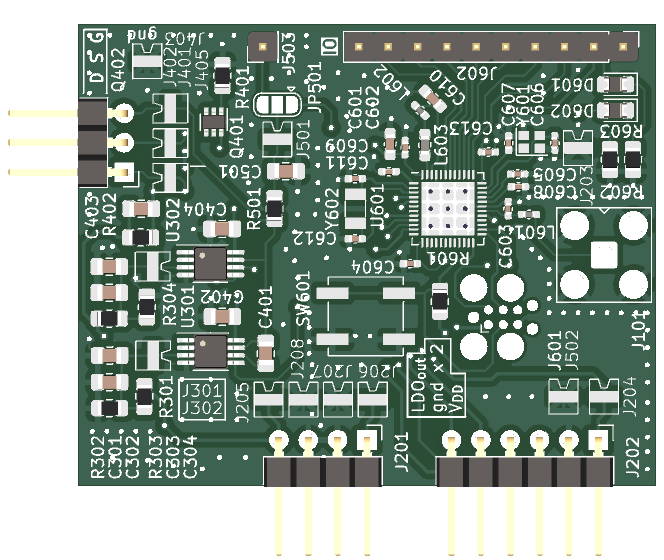
\includegraphics[width=\textwidth]{sensorBord}
        \caption{De ISFET uitlezende PCB.}
        \label{fig:sensorPCB}
    \end{subfigure}
    \hfill
    \begin{subfigure}[b]{0.60\textwidth}
        \centering
        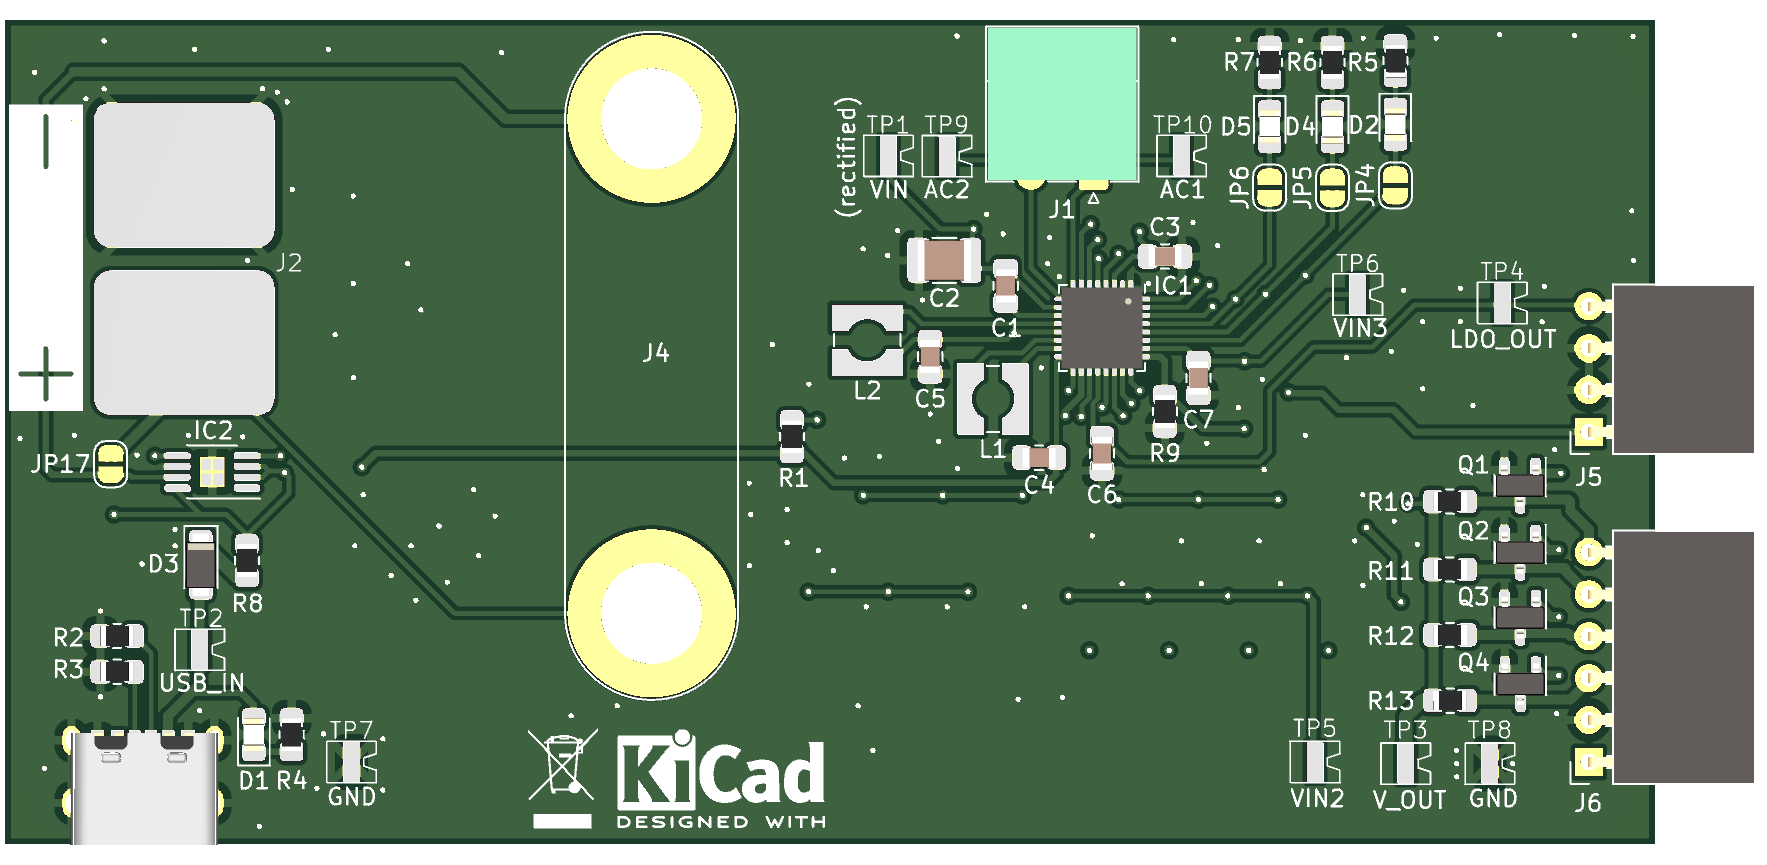
\includegraphics[width=\textwidth]{powerandharvest}
        \caption{De voeding en harvesting PCB.}
        \label{fig:powerPCB}
    \end{subfigure}
    \caption{De gemaakte PCB's.}
    \label{fig:PCBs}
\end{figure}


\subsection{Temperatuursensor}

Er is nog niks ontworpen voor het meten van de temperatuur van de te meten oplossing. De \mcu heeft echter wel een ingebouwde temperatuursensor.
Deze kan gebruikt worden om te compenseren voor veranderingen in temperatuur, zolang de temperatuur van de \mcu niet te veel afwijkt van de temperatuur van de te meten oplossing.


